\subsection{Example}%
\label{subsec:kgraph_example}
An example \ac{kgraph} can be visualized in \Cref{fig:kgraph_example}, the parameterization of edges is displayed and the object that the edge controls as image. For clarification, the connected left part with image of the point robot on the center node has 3 outgoing edges that describe robot driving. The connected part on the right with an image of the point robot and the green box on the center node has 2 outgoing edges that describe robot pushing against the green box.\bs

\begin{figure}[H]
    \centering
    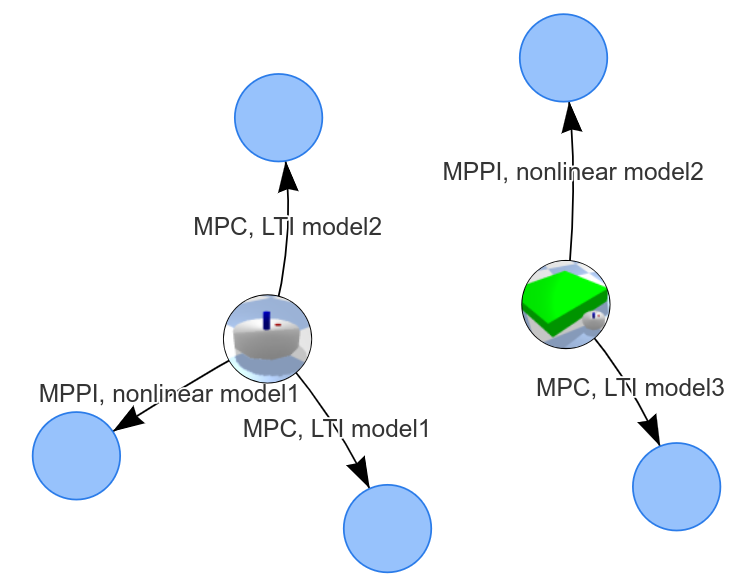
\includegraphics[width=10cm]{figures/kgraph_example}
    \caption{\ac{kgraph} with 3 edges on robot driving, and 2 edges for pushing the green box.}%
    \label{fig:kgraph_example}
\end{figure}

The edges in the figure above display only the edge parameterization, but store more information, mainly the success factor. The blue nodes serve a small purpose, making sure edges can point to a node. The blue nodes could fulfill a larger purpose, that is describing which actuators the edge can control. For example, a mobile robot with robot arm attached can have a set of controllers that only drive the base, a set of controllers that only steer the robot arm and a set that controls both the base and robot arm. In such cases the blue nodes describe which part can of the robot can be actuated. The controllers considered in this thesis control every actuator of the robot, resulting in the blue nodes serving such a small purpose.\bs
